\section{Introduction}
\label{sec:introduction}

An increasing number of swarm applications rely on heavy computation tasks, such
machine learning (ML). For example, Microsoft SeeingAI~\cite{seeingai} is a
talking camera for the blind and low vision community that describes nearby
people, text, objects. Wearable cognitive assistant~\cite{ha2014towards} uses
wearable devices, such as Google Glass, for deep cognitive assistance, e.g.,
offering hints for social interaction via real-time scene analysis.

While there is a staggering collection of research focusing on model
\textit{training} for these tasks, for swarm applications, they perform the
\textit{inference} step of machine learning: use trained models to make a
prediction given an input, such as visual~\cite{googlelens, ha2014towards,
  seeingai}, audio~\cite{alexa, applesiri, cortana}, and sensory
information~\cite{laput2017synthetic, lu2010jigsaw}. Inference has received
relatively little attention, especially on edge and end devices.

One important challenge for inference is to bound the response time, which
affects user experience significantly in these human-in-the-loop
systems. Previous usability studies~\cite{nielsen1994usability,
  schneiderman1998designing} have measured the effect of different end-to-end
latencies:

\begin{itemize}[noitemsep, topsep=5pt]
\item 100 ms gives the feeling of instantaneous response.
\item 1 second keeps the user's flow of thought but users can sense the delay.
\item A few seconds' delay creates an unpleasant user experience.
\end{itemize}

Achieving bounded response times (BRT) on swarm devices has remained
challenging. Swarm devices are extremely heterogeneous and many are resource
constrained (see \autoref{tab:embedded}). Many heavy computations are simply
beyond the capabilities of cheap end devices. State-of-the-art computer vision
algorithms, such as object detection, easily take several seconds on modern
smartphones~\cite{chen2015glimpse}.

To compensate resource-constrained devices, prior work explores
offloading~\cite{chun2011clonecloud,cuervo2010maui} to the cloud or the edge
that hosts machine learning models and performs heavy computation. Despite their
powerful computing capability and more available resources, e.g., special
hardware like GPU and TPU~\cite{jouppi2017datacenter}, these platforms suffer
from increased network latency and service overload (\autoref{fig:edge}). As a
result, they are often unable to meet latency goals consistently.

Another technique for low latency is to use redundant requests. By initiating
multiple requests across a diverse set of resources and using the first result
that completes, redundancy is effective to address the variability in network
delays~\cite{gordon2015accelerating, vulimiri2013low} and slow servers (known as
straggler mitigation in the cloud~\cite{dean2013tail,
  ananthanarayanan2013effective}). However, existing works treat these resources
equally and executes the same task on each platform, a poor match for the
heterogeneous swarm space.

We make the observation that for a particular task, there are many options:
different algorithms or tunable parameters for the same algorithm. These options
result in different processing times and accuracy. If we can adapt the
computation by choosing an option that matches the capability of the device, we
can achieve bounded response times.

The idea of adapting to platforms is illustrated in \autoref{fig:dr}. It builds
on top of redundancy but addresses (or leverages) the heterogeneity of swarm
platforms.  On-device processing can use a simple algorithm if the device is
resource constrained. The device also sends redundant requests to other servers,
e.g., the edge and/or the cloud. Each request contains a service-level objective
(SLO) that describes the deadline and accuracy demand. Upon receiving the
request, the server would admit or reject the request based on the network
delays and its workload. Because of the redundancy, rejection is fine. This is
different from traditional web serving where the server is the single point of
source. At last, the device would use the first response that completes.

\begin{figure}
  \centering
  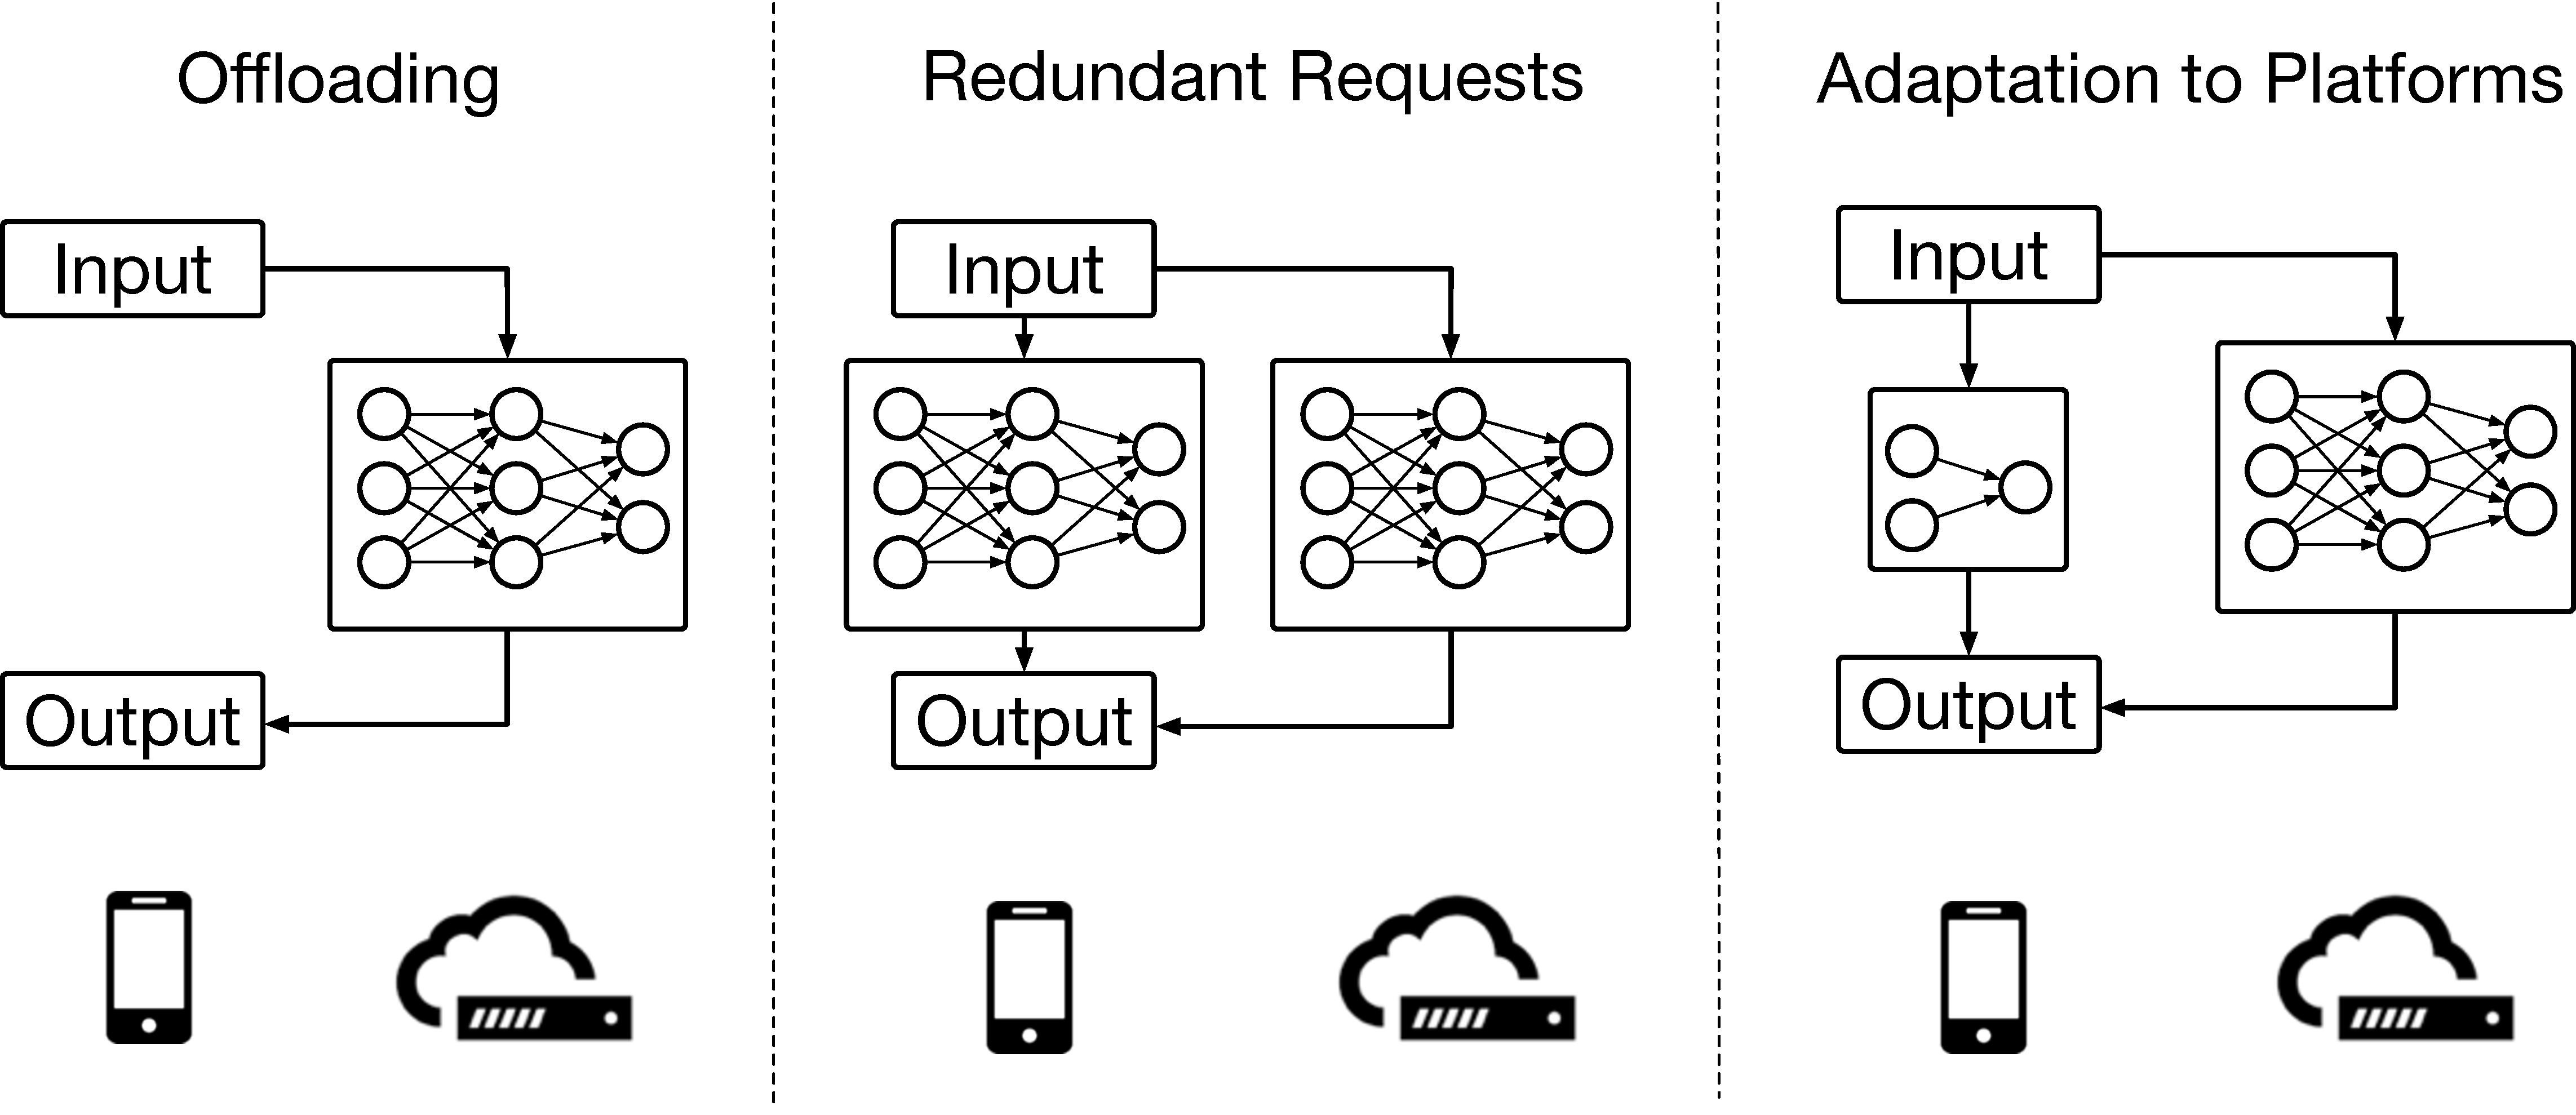
\includegraphics[width=0.8\columnwidth]{figures/dr.pdf}
  \caption{Illustration of offloading, redundant requests and differential
    redundancy.}
  \label{fig:dr}
\end{figure}

%% //////////////////////////////

The key to enable adaptation, which is also the challenge, lies in building an
accurate performance model that characterized the processing times and accuracy
trade-off for a particular task.

This adaptation technique is orthogonal to existing system solutions, such as
scale-out, scale-up, caching, or batching. Because it is an application-aware
approach, the adaptation requires knowledge from the application developer.

Efficient profiling to find the performance model. In order to explore the
trade-off space, we take a data-driven approach to learn the relationship
between inference accuracy and processing times for each algorithm and different
parameters for individual platforms. We call this process ``profiling'' and its
goal is to find Pareto-optimal configurations (algorithm and parameter) as the
performance model.

Profiling with an exhaustive search may not be feasible for some algorithms due
to their large parameter space. In these cases, we use a statistical method,
Bayesian Optimization (BO), to model the relationship as a black-box function
and only searches for near-optimal configurations.

Profiling for all hardware platforms is not feasible due to the large space and
availability of the hardware at development time. We observe that the profile
can be easily transferred across platforms with linear transformation.

We make the following contributions in this chapter with \brt{}:

\begin{itemize}

\item The proposed Bayesian Optimization (BO) for profiling, significantly
  outperforms previous approaches with random search or coordinate/greedy
  approach.
\item We empirically validate the profile transfer to address heterogeneous
  capabilities across swarm platforms.

\end{itemize}

% \begin{figure*}
%   \centering
%   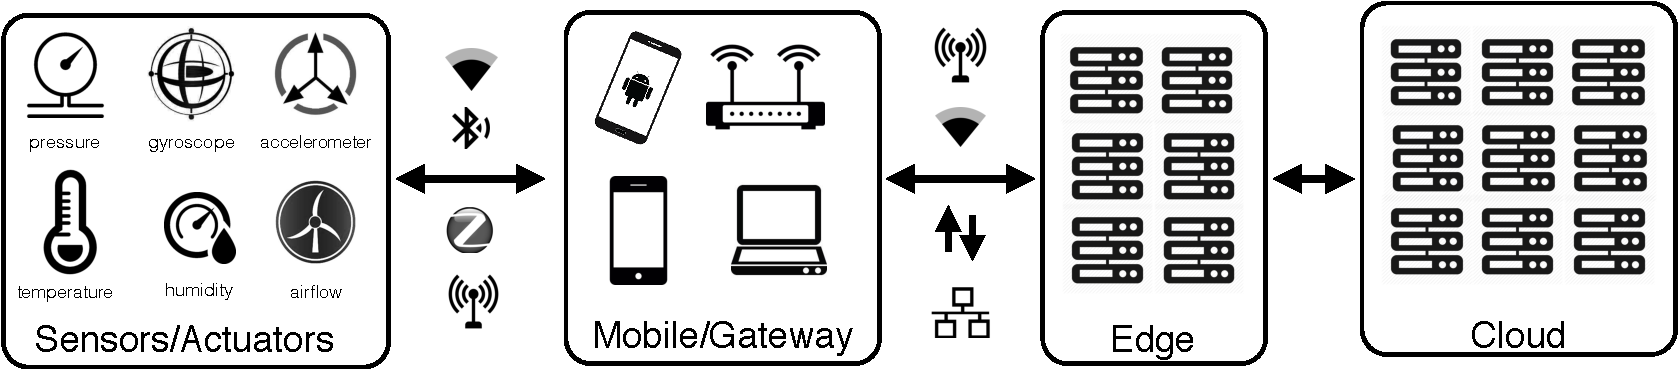
\includegraphics[width=\textwidth]{figures/platforms}
%   \label{fig:options}
%   \caption{Platforms}
% \end{figure*}

%%% Local Variables:
%%% mode: latex
%%% TeX-master: "../compute"
%%% End:
